\documentclass{article}
\usepackage[T1]{fontenc}
\usepackage{lmodern}
\usepackage{graphicx}
\usepackage{amsmath,amssymb}
\usepackage[a4paper,margin=2cm]{geometry}
\usepackage[absolute,overlay]{textpos}
\setlength{\TPHorizModule}{1mm}
\setlength{\TPVertModule}{1mm}
\usepackage[indonesian]{babel}
\usepackage{hyperref}
\setlength{\emergencystretch}{2em}
% unit: Halaman 40

\begin{document}

% === Halaman 40 (llm) ===

\section*{InvSubBytes()}

\vspace{160.38mm}

\begin{itemize}
    \item $InvSubBytes()$ sama seperti di dalam $SubBytes()$, hanya saja S-box yang digunakan adalah inversi dari S-box
\end{itemize}

\vspace{10mm}

\centerline{Gambar 6.27 Inversi S-box di dalam Rijndael}

% deskripsi: Tabel inversi S-box yang digunakan dalam algoritma enkripsi Rijndael/AES, menampilkan pemetaan nilai heksadesimal dari indeks baris dan kolom ke nilai hasil inversi.
% bbox normalisasi: [0.1500, 0.3300, 0.8300, 0.8700]
\begin{textblock*}{142.80mm}(31.50mm,98.01mm)
\noindent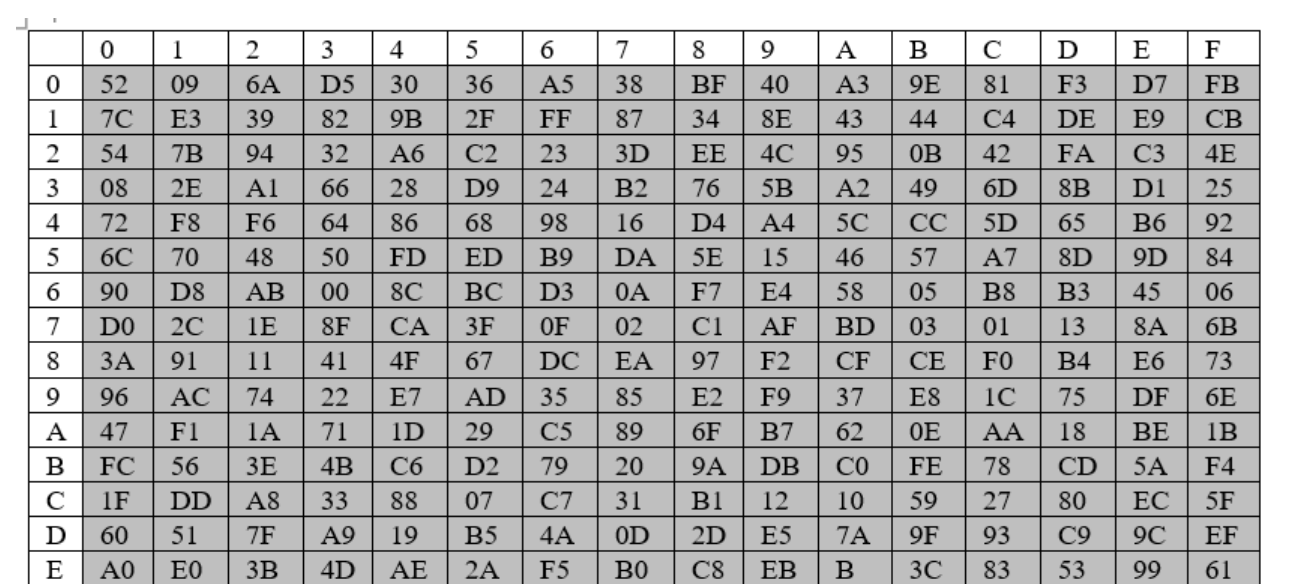
\includegraphics[width=142.80mm,height=160.38mm]{../../images/llm/page_040_img_01.png}%
\end{textblock*}

\end{document}
